\documentclass[11pt,a4paper]{article}

\usepackage[margin=2.3cm]{geometry}
\usepackage{amsmath,amssymb}
\usepackage{graphicx}
\usepackage{booktabs}
\usepackage{xcolor}
\usepackage{enumitem}
\usepackage[hidelinks]{hyperref}
\usepackage{caption}
\usepackage{float}

\emergencystretch=1.5em
\captionsetup{font=small,labelfont=bf,width=.92\textwidth}
\setlength{\parskip}{4pt plus 1pt}
\setlength{\parindent}{0pt}

\newcommand{\code}[1]{\texttt{#1}}
\newcommand{\bst}[1]{\textbf{#1}}

\title{DUST on the $K{=}32$ code-carried model:\\ the 500-step $\sigma \times$ \code{dust\_lr\_scale} grid\\[2pt]
\large Research note}
\author{}
\date{2026-10-22.}

\begin{document}
\maketitle
\vspace{-2em}

Single runs, seed 1337; the encoder arm and the baseline trained on new\_york
(8$\times$ RTX 5090), the backprop arm on georgia (8$\times$ A100).

% ============================================================
\section{Setup}
% ============================================================

The model is the $K{=}32$ code-carried hard Top-32 model of
\path{docs/kj-vs-hard-topk-code-residual.tex}
(\path{configs/cr_kj/ma_cr_hard_k32_pnorm.yaml}): 8 blocks of width 768,
abs-TopK over $N = 1536$ features at \code{residual\_out} of every block, the
code carried between blocks, post-norm, magnitude--direction (MD) decoupling,
batch $96 \times 512$ tokens, a 20k-step cosine schedule with 500 warmup steps.

Every DUST run (\path{configs/cr_dust/hp500/}, method in
\path{docs/dust-topk.md}) adds the DUST bottleneck optimization: the $J = 480$
pool receives the noise, population 128 (16 draws per bottleneck), schedule
$[1, 1]$ (every other optimizer step a DUST step), $\gamma = 0$, gradient
scale 1, a separate optimizer for the DUST steps sharing the MD
parameterization, and no gradient clipping. The grid is \code{dust\_target}
$\in \{\text{encoder}, \text{backprop}\}$ $\times$ $\sigma \in \{0.03, 0.1, 0.3,
0.9\}$ $\times$ \code{dust\_lr\_scale} $\in \{1, 10, 30, 100, 300\}$. Each run
trains 500 steps of the unchanged 20k-step schedule, so the window lies inside
the LR warmup ($1.2 \cdot 10^{-6}$ to $6 \cdot 10^{-4}$; the DUST steps use that
value times \code{dust\_lr\_scale}), with validation every 50 steps on 40
batches of 24 windows.

The baseline is the same model trained with the same settings and no DUST
steps (\path{ny_hp500_hard_k32}); the original madrid run of the model
(gradient clipping at 1.0) is quoted for reference.

% ============================================================
\section{Encoder target}
% ============================================================

\begin{figure}[H]\centering
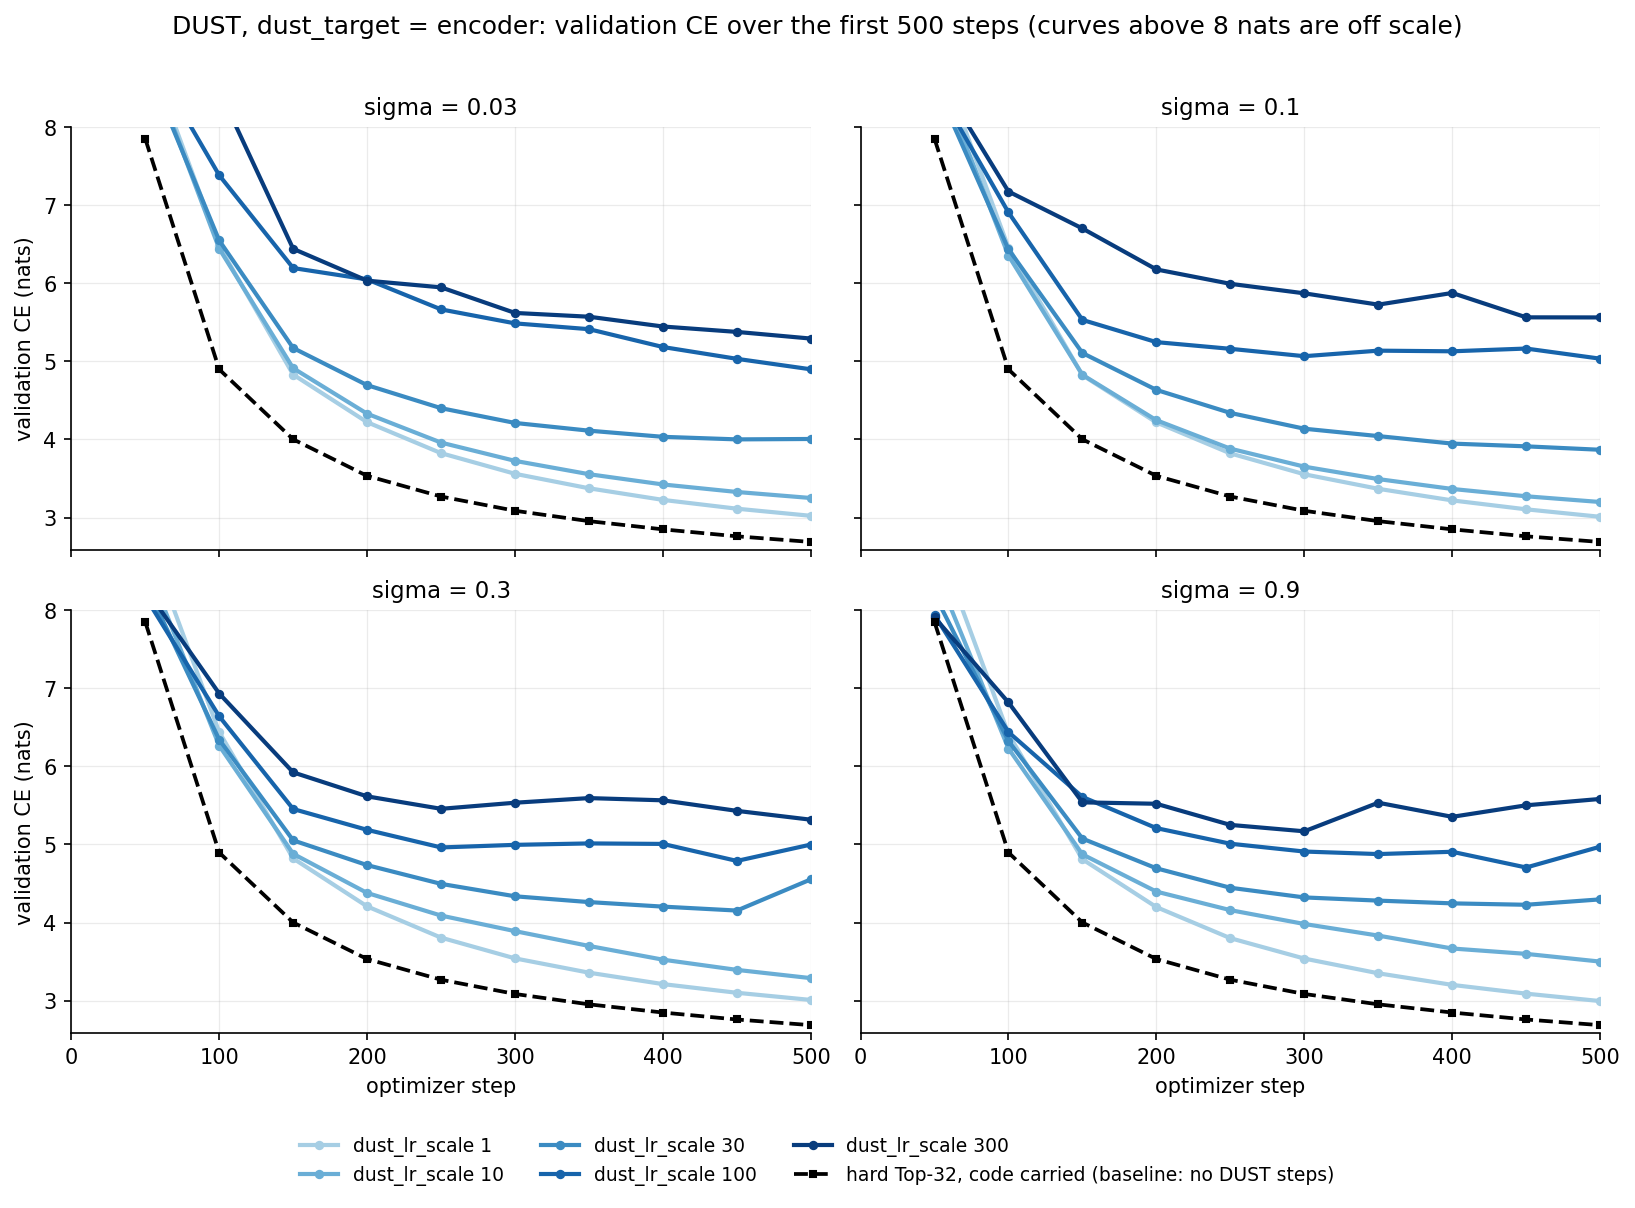
\includegraphics[width=\textwidth]{figures/hp500_val_encoder.png}
\caption{\code{dust\_target = encoder}: validation CE over the first 500 steps,
one panel per $\sigma$, one curve per \code{dust\_lr\_scale} (one hue, light
to dark with the multiplier); dashed black, the hard Top-32 baseline. Curves
above 8 nats are off scale.}
\end{figure}

Validation CE at step 500 (bold: the best cell):

\begin{center}\small
\begin{tabular}{lccccc}
\toprule
$\sigma \,\backslash\, $\code{dust\_lr\_scale} & 1 & 10 & 30 & 100 & 300 \\
\midrule
$0.03$ & 3.0220 & 3.2500 & 4.0055 & 4.8971 & 5.2906 \\
$0.1$  & 3.0096 & 3.1989 & 3.8673 & 5.0334 & 5.5611 \\
$0.3$  & 3.0101 & 3.2891 & 4.5535 & 4.9989 & 5.3168 \\
$0.9$  & \bst{2.9957} & 3.5009 & 4.2972 & 4.9715 & 5.5825 \\
\midrule
hard Top-32 baseline (no DUST steps, same settings) & 2.6875 & & & & \\
hard Top-32, the original madrid run (clipping 1.0) & 2.6846 & & & & \\
\bottomrule
\end{tabular}
\end{center}

% ============================================================
\section{Backprop target}
% ============================================================

\begin{figure}[H]\centering
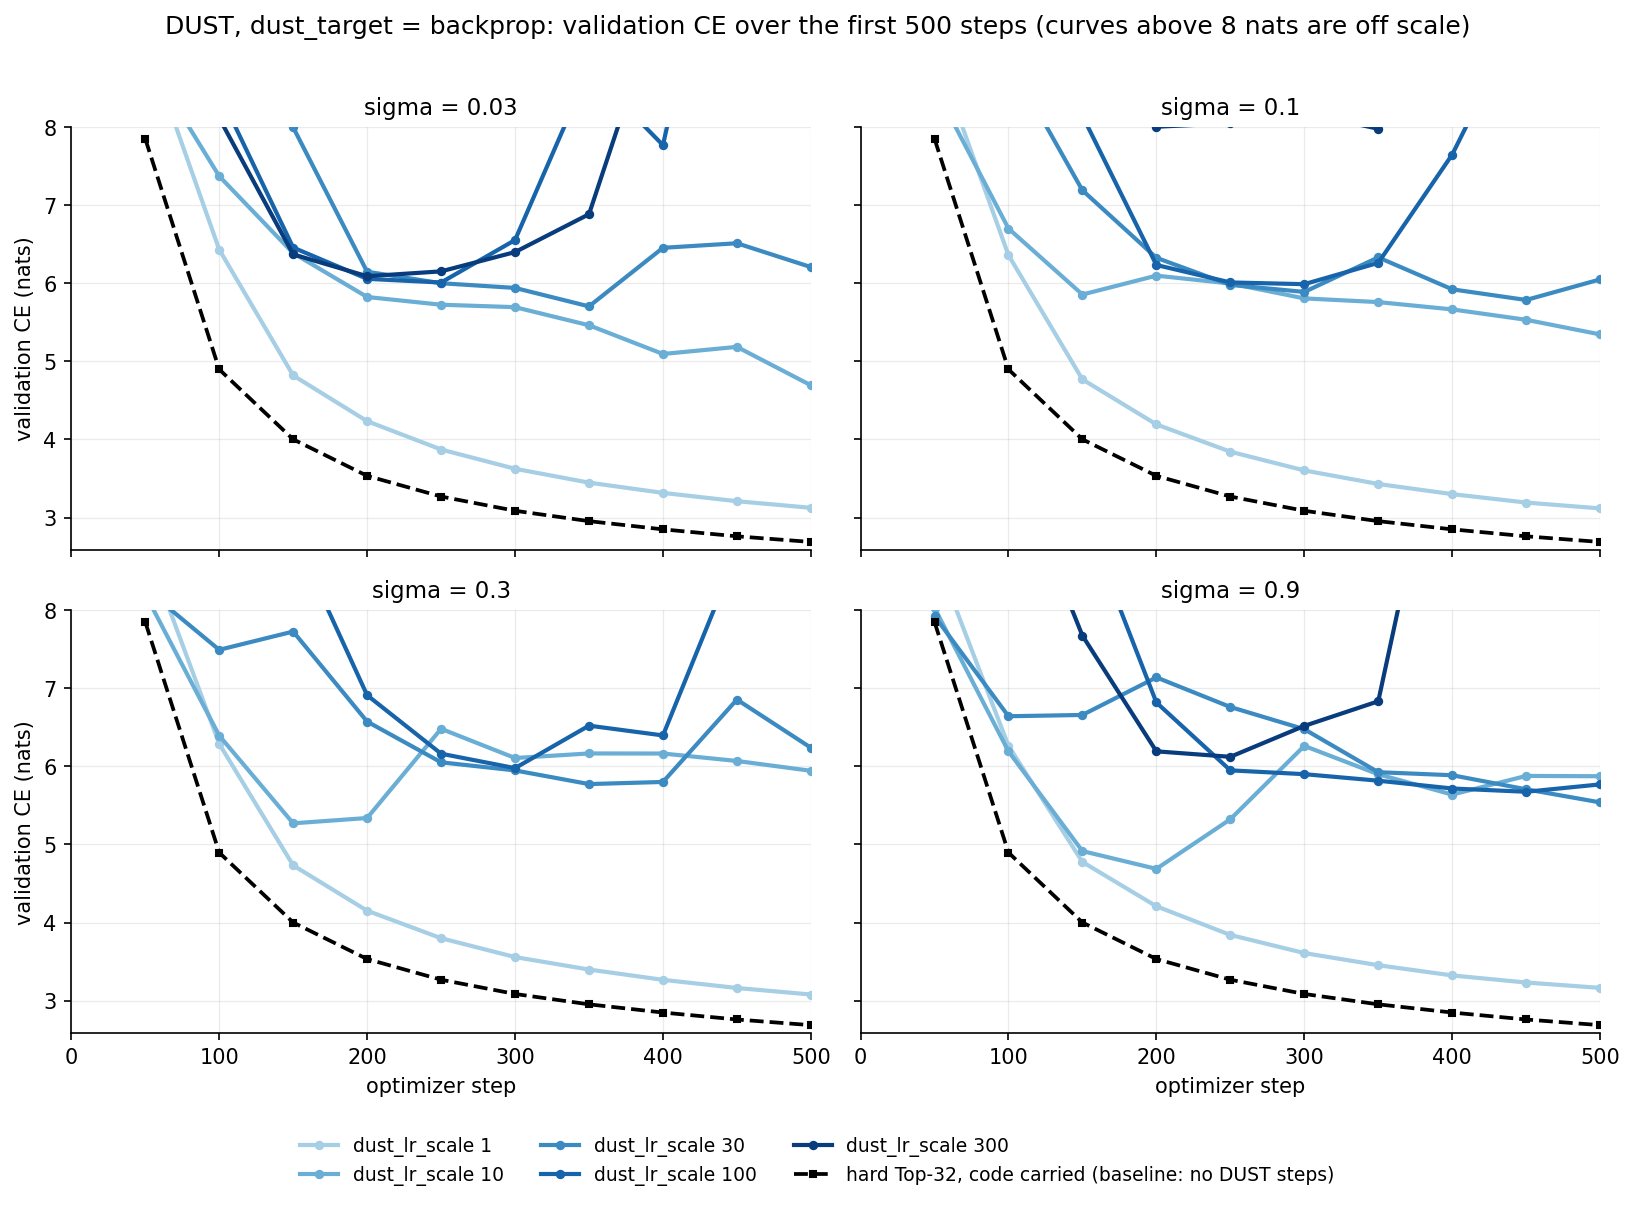
\includegraphics[width=\textwidth]{figures/hp500_val_backprop.png}
\caption{\code{dust\_target = backprop}: the same layout. Curves above 8
nats are off scale.}
\end{figure}

Validation CE at step 500:

\begin{center}\small
\begin{tabular}{lccccc}
\toprule
$\sigma \,\backslash\, $\code{dust\_lr\_scale} & 1 & 10 & 30 & 100 & 300 \\
\midrule
$0.03$ & 3.1246 & 4.6930 & 6.2055 & 13.0487 & 9.7345 \\
$0.1$  & 3.1169 & 5.3437 & 6.0478 & 8.8164 & 9.9774 \\
$0.3$  & \bst{3.0794} & 5.9428 & 6.2382 & 11.9248 & 9.6194 \\
$0.9$  & 3.1646 & 5.8732 & 5.5386 & 5.7687 & 9.2661 \\
\midrule
hard Top-32 baseline (no DUST steps, same settings) & 2.6875 & & & & \\
hard Top-32, the original madrid run (clipping 1.0) & 2.6846 & & & & \\
\bottomrule
\end{tabular}
\end{center}

% ============================================================
\section{Results}
% ============================================================

No cell reaches the baseline. In both arms the validation CE at step 500
rises monotonically with \code{dust\_lr\_scale}, and the multiplier 1 is the
best value at every $\sigma$: 2.996 to 3.022 in the encoder arm, 0.31 to 0.33
nats above the baseline, and 3.08 to 3.16 in the backprop arm. The dependence
on $\sigma$ is weak at the multiplier 1 (a spread of 0.03 nats in the encoder
arm and 0.09 in the backprop arm) and does not change the ordering by the
multiplier anywhere.

The two targets differ in how the larger multipliers fail. In the encoder arm
the curves keep descending at every setting, only more slowly and from a
higher level as the multiplier grows; at 100 and 300 they plateau near 5 to
5.6 nats within the window. In the backprop arm, where the estimate is
backpropagated to every parameter before the gate inputs, every multiplier
from 10 on stalls near 5 to 6 nats, and 100 and 300 diverge at every $\sigma$
(final values of 5.8 to 13 nats), with the pre-activation scale growing by
orders of magnitude within the first tens of steps.

Within the first 500 steps the DUST steps therefore cost against hard steps
at every setting of the grid, least when the DUST learning rate is the
schedule's own, and the encoder target is less harmful than the backprop
target at every $\sigma$ and multiplier.

% ============================================================
\section{Sigma sweep at population 1024}
% ============================================================

\code{dust\_lr\_scale} 1, population 1024 (128 draws per bottleneck, eight
times the grid's), both targets, the four $\sigma$ values, otherwise the
grid's settings; all eight runs on new\_york.

\begin{figure}[H]\centering
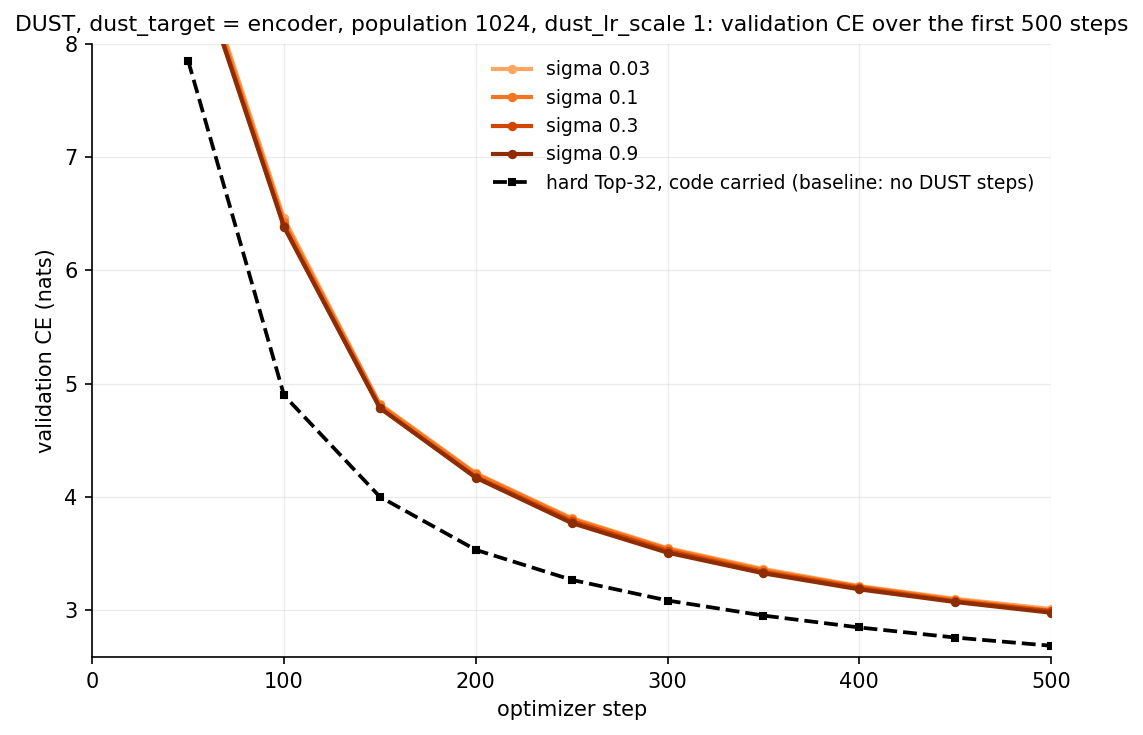
\includegraphics[width=.72\textwidth]{figures/hp500_p1024_val_encoder.png}
\caption{Population 1024, \code{dust\_target = encoder}: validation CE over
the first 500 steps, one curve per $\sigma$ (one hue, light to dark with
$\sigma$); dashed black, the hard Top-32 baseline.}
\end{figure}

\begin{figure}[H]\centering
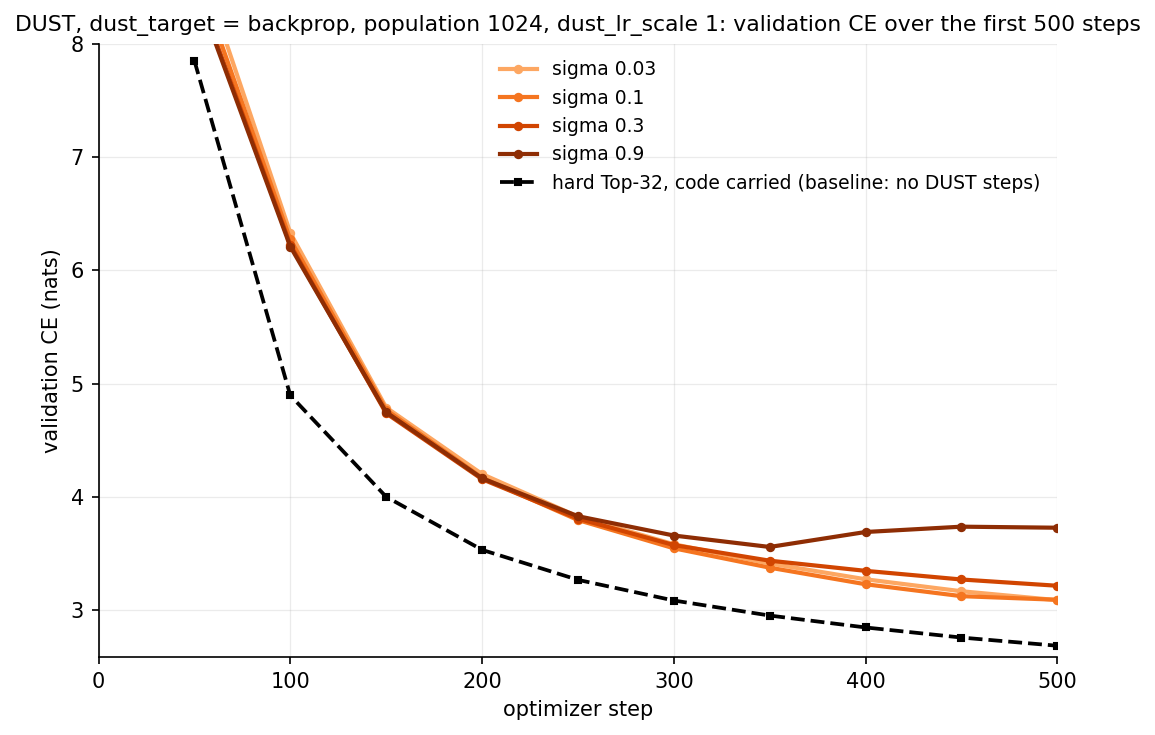
\includegraphics[width=.72\textwidth]{figures/hp500_p1024_val_backprop.png}
\caption{Population 1024, \code{dust\_target = backprop}: the same layout.}
\end{figure}

Validation CE at step 500 (population 128 at \code{dust\_lr\_scale} 1 in
parentheses):

\begin{center}\small
\begin{tabular}{lcccc}
\toprule
\code{dust\_target} $\backslash\, \sigma$ & $0.03$ & $0.1$ & $0.3$ & $0.9$ \\
\midrule
encoder  & 3.0117 (3.0220) & 2.9975 (3.0096) & 2.9923 (3.0101) & \bst{2.9790} (2.9957) \\
backprop & 3.0896 (3.1246) & 3.0930 (3.1169) & 3.2166 (3.0794) & 3.7286 (3.1646) \\
\midrule
hard Top-32 baseline (no DUST steps, same settings) & 2.6875 & & & \\
hard Top-32, the original madrid run (clipping 1.0) & 2.6846 & & & \\
\bottomrule
\end{tabular}
\end{center}

Eight times the population lowers the encoder arm's CE at step 500 by 0.010
to 0.018 nats at every $\sigma$, and the four curves are indistinguishable
until the last 100 steps, where they order by $\sigma$ with the largest best.
The backprop arm improves by 0.02 to 0.04 at $\sigma = 0.03$ and $0.1$ and
worsens at $0.3$ and $0.9$, where the curves turn upward after step 350
($\sigma = 0.9$ ends at 3.73). The gap to the baseline, 0.29 nats in the
encoder arm at best, is therefore not a matter of the estimate's variance at
this population: the estimate's variance is eight times smaller and the gap
moved by a few hundredths.

% ============================================================
\section{Without MD decoupling}
% ============================================================

The hard Top-32 run and the population-1024 $\sigma$ sweep
(\code{dust\_lr\_scale} 1, both targets) repeated with \code{model.decouple
= false} and \code{model.md\_init = true}: the initialization is the same,
only the optimizer changes, from the decoupled one (directions on fixed-norm
spheres, learnable gains, no weight decay) to ordinary AdamW with weight
decay 0.1, the convention of \path{docs/md-init-vs-decoupling.tex}. The hard
run and the $\gamma = 0$ sweep on georgia, the $\gamma = 0.99$ sweep on
new\_york; checkpoints at steps 250 and 500.

\begin{figure}[H]\centering
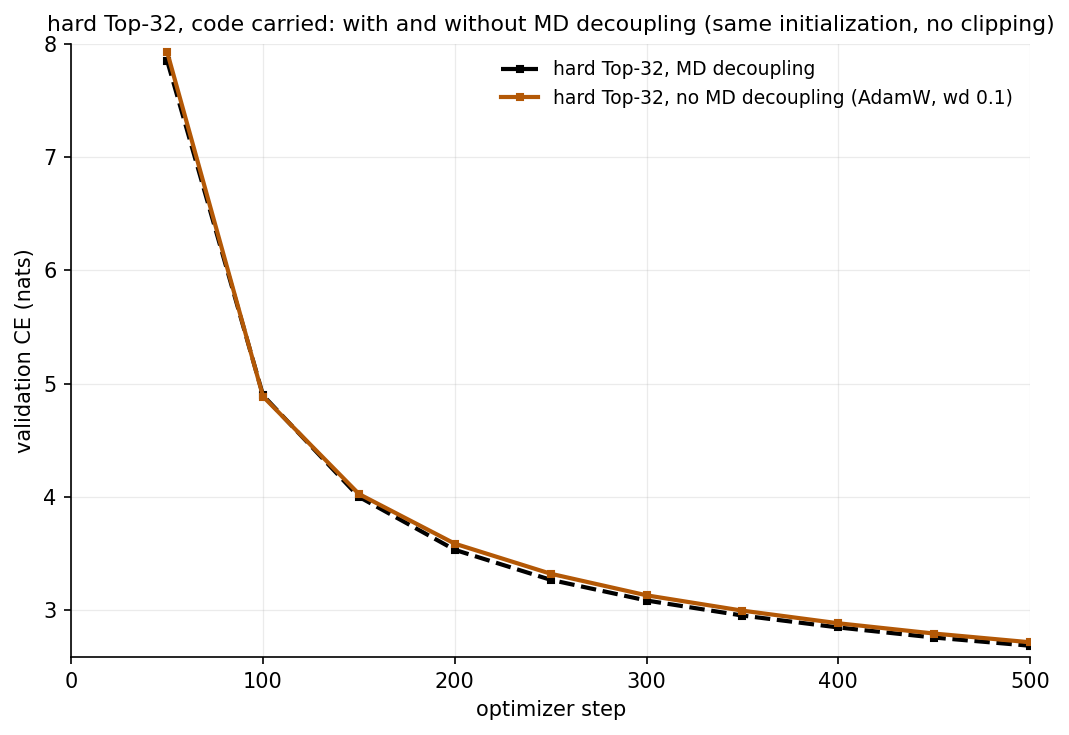
\includegraphics[width=.72\textwidth]{figures/hp500_hard_md_vs_nomd.png}
\caption{Hard Top-32, code carried, with (dashed black) and without (solid)
MD decoupling: same initialization, no clipping, validation every 50 steps.}
\end{figure}

\begin{center}\small
\begin{tabular}{lc}
\toprule
run & validation CE at step 500 \\
\midrule
hard Top-32, MD decoupling & 2.6875 \\
hard Top-32, no MD decoupling (AdamW, weight decay 0.1) & 2.7181 \\
\bottomrule
\end{tabular}
\end{center}

The two hard runs coincide to step 150 and separate by 0.03 to 0.06 nats from
step 200 on; at step 500 the decoupled optimizer is 0.031 nats ahead.

\subsection*{$\gamma = 0$}

\begin{figure}[H]\centering
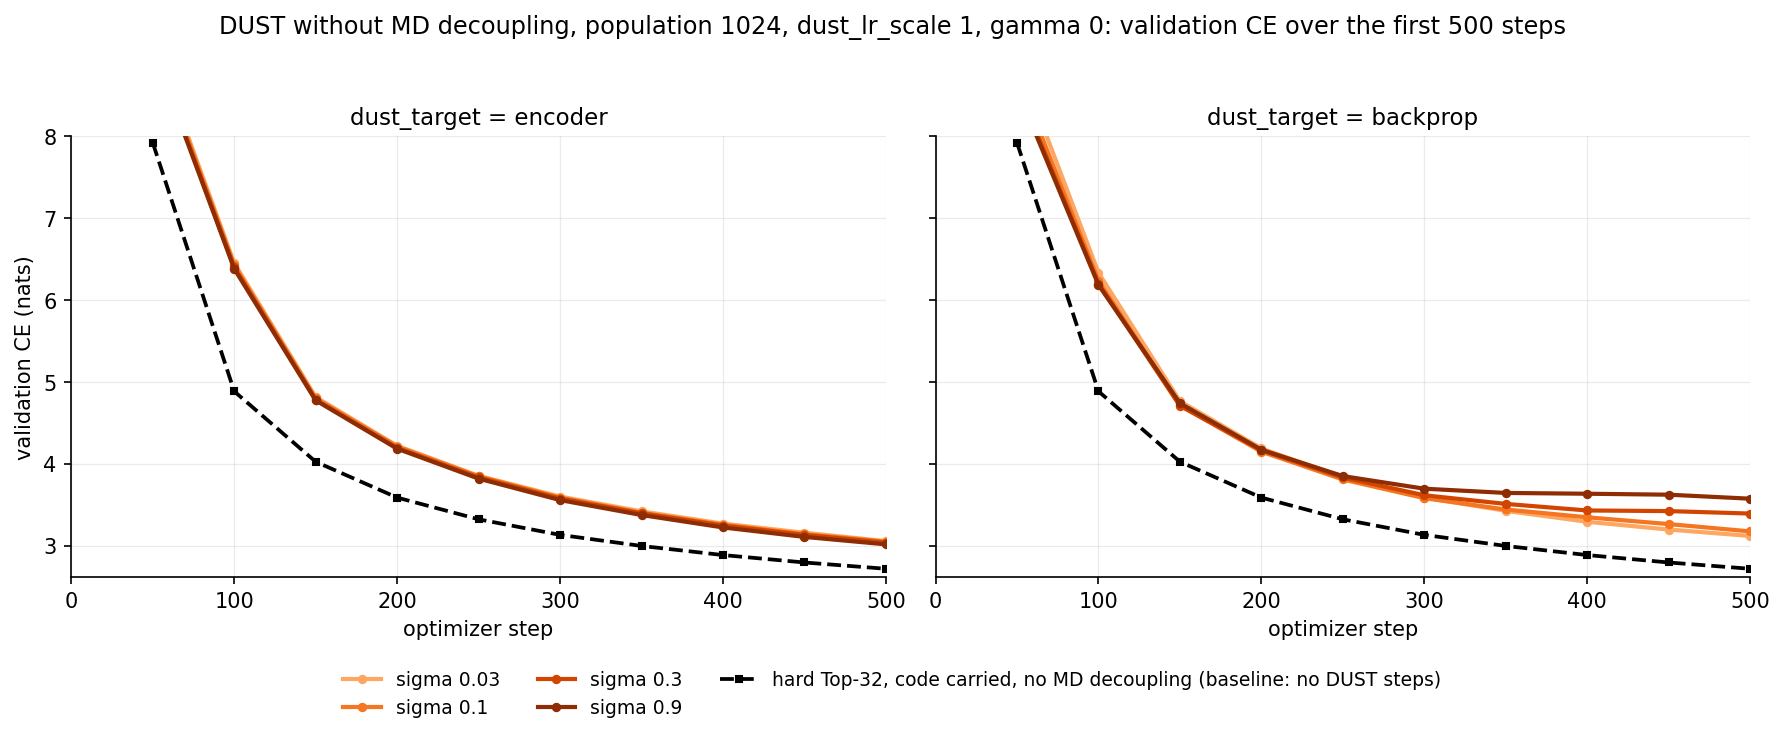
\includegraphics[width=\textwidth]{figures/hp500_p1024_nomd_g0_val.png}
\caption{DUST without MD decoupling, population 1024, \code{dust\_lr\_scale}
1, $\gamma = 0$: encoder target left, backprop target right, one curve per
$\sigma$; dashed black, the hard Top-32 run without decoupling.}
\end{figure}

Validation CE at step 500, without MD decoupling (with MD, from the sweep of
Section~5, in parentheses):

\begin{center}\small
\begin{tabular}{lcccc}
\toprule
\code{dust\_target} $\backslash\, \sigma$ & $0.03$ & $0.1$ & $0.3$ & $0.9$ \\
\midrule
encoder  & 3.0558 (3.0117) & 3.0492 (2.9975) & 3.0369 (2.9923) & \bst{3.0163} (2.9790) \\
backprop & 3.1192 (3.0896) & 3.1748 (3.0930) & 3.3926 (3.2166) & 3.5744 (3.7286) \\
\midrule
hard Top-32, no MD decoupling (no DUST steps, same settings) & 2.7181 & & & \\
\bottomrule
\end{tabular}
\end{center}

Removing the decoupling moves the DUST runs by about as much as it moves the
baseline: the encoder arm ends 0.30 to 0.34 nats above the no-MD hard run
(0.29 to 0.32 above the MD hard run with decoupling), ordered by $\sigma$
with the largest best and the four curves indistinguishable to step 400. The
backprop arm ends 0.40 to 0.86 nats above it; its curves separate after step
250 and flatten for $\sigma = 0.3$ and $0.9$, which end at 3.39 and 3.57
(with decoupling, $\sigma = 0.9$ turned upward to 3.73). The gap between
DUST and the hard model is therefore not a property of the decoupled
optimizer.

\subsection*{$\gamma = 0.99$}

The same eight runs with \code{dust\_gamma} $= 0.99$: a token's noise is
rewarded with its own loss change plus the discounted loss changes of the
later tokens.

\begin{figure}[H]\centering
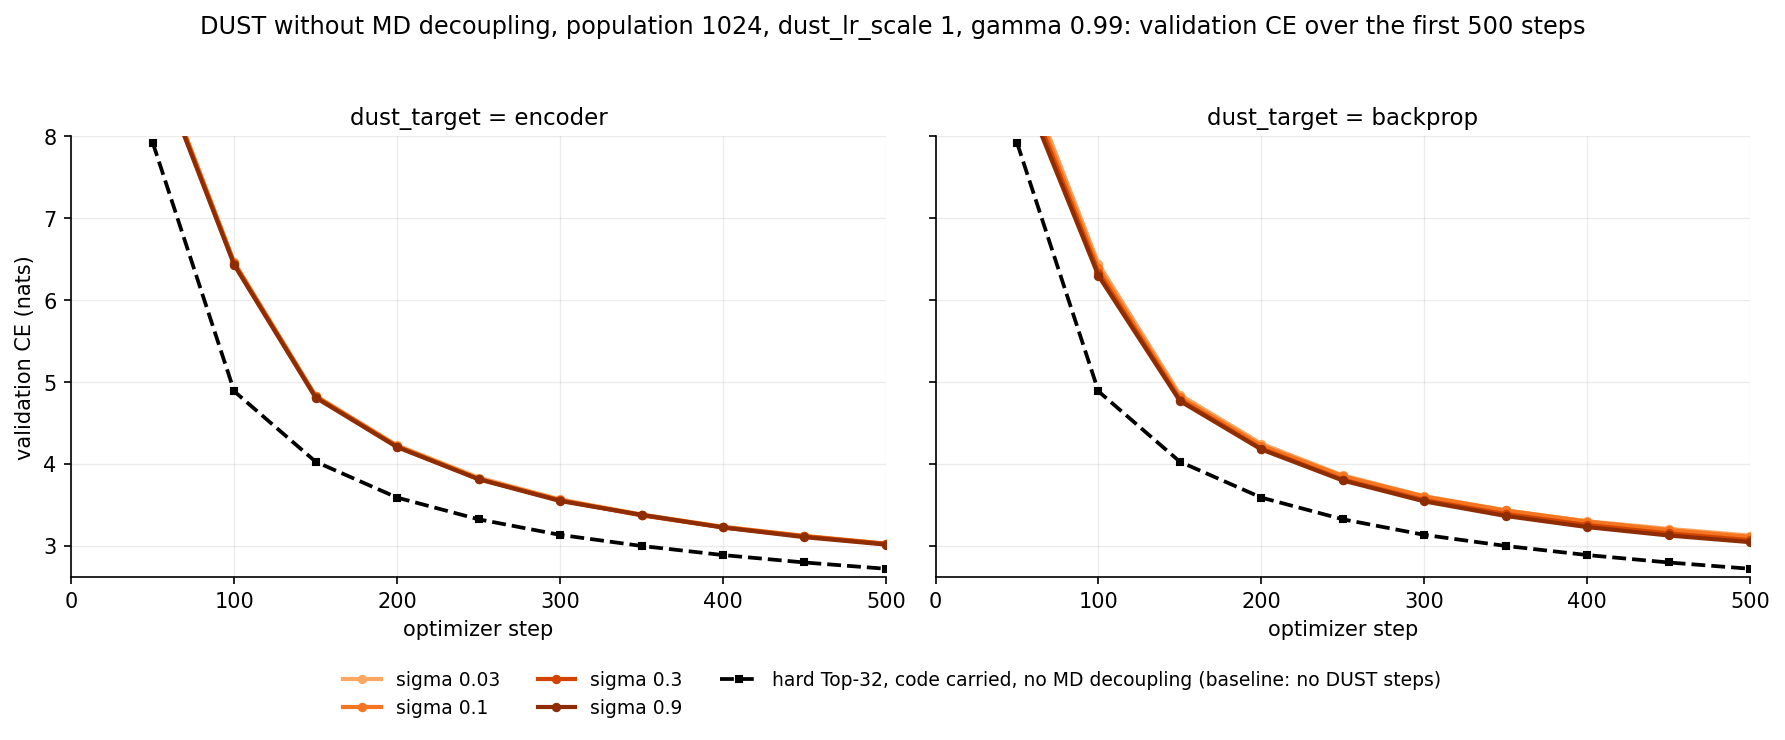
\includegraphics[width=\textwidth]{figures/hp500_p1024_nomd_g0p99_val.png}
\caption{As above, $\gamma = 0.99$.}
\end{figure}

Validation CE at step 500 ($\gamma = 0$ in parentheses):

\begin{center}\small
\begin{tabular}{lcccc}
\toprule
\code{dust\_target} $\backslash\, \sigma$ & $0.03$ & $0.1$ & $0.3$ & $0.9$ \\
\midrule
encoder  & 3.0248 (3.0558) & 3.0193 (3.0492) & 3.0241 (3.0369) & \bst{3.0139} (3.0163) \\
backprop & 3.1229 (3.1192) & 3.1082 (3.1748) & 3.0665 (3.3926) & 3.0437 (3.5744) \\
\midrule
hard Top-32, no MD decoupling (no DUST steps, same settings) & 2.7181 & & & \\
\bottomrule
\end{tabular}
\end{center}

The discounted credit changes the backprop arm most: the flattening at
$\sigma = 0.3$ and $0.9$ disappears (3.39 to 3.07 and 3.57 to 3.04), the arm
is now ordered by $\sigma$ with the largest best, and it ends within 0.03 of
the encoder arm. The encoder arm gains 0.01 to 0.03 nats at $\sigma = 0.03$
to $0.3$ and nothing at $0.9$, with its four curves again on top of one
another. Both arms stay 0.30 to 0.40 nats above the hard run. The per-draw
signal-to-noise ratio of the estimate (\code{dust/snr}, defined in
\path{docs/dust-topk.md}) is 0.088 to 0.091 in every one of these sixteen
cells at step 500, independent of $\sigma$, target and $\gamma$, so at 128
draws per bottleneck the population estimate has a per-token signal-to-noise
ratio of about 1.

% ============================================================
\section{Runs on Drive}
% ============================================================

\begin{itemize}[leftmargin=1.4em]
\item Encoder arm, new\_york: \path{gdrive:weight-sparsity/runs_new_york/ny_hp500_enc_sg<s>_lr<l>}
  for \path{<s>} $\in$ \{\path{0p03}, \path{0p1}, \path{0p3}, \path{0p9}\} and
  \path{<l>} $\in$ \{1, 10, 30, 100, 300\}, twenty runs.
\item Baseline, new\_york: \path{gdrive:weight-sparsity/runs_new_york/ny_hp500_hard_k32}.
\item Population-1024 sweep, new\_york: \path{gdrive:weight-sparsity/runs_new_york/ny_hp500_<a>_p1024_sg<s>_lr1}
  for \path{<a>} $\in$ \{\path{enc}, \path{bp}\}, eight runs.
\item Backprop arm, georgia: \path{gdrive:weight-sparsity/runs_georgia/ga_hp500_bp_sg<s>_lr<l>},
  the same twenty cells.
\item Without MD decoupling, georgia: \path{gdrive:weight-sparsity/runs_georgia/ga_hp500_hard_k32_nomd}
  and \path{gdrive:weight-sparsity/runs_georgia/ga_hp500_<a>_p1024_nomd_sg<s>_lr1}, eight runs.
\item Without MD decoupling, $\gamma = 0.99$, new\_york:
  \path{gdrive:weight-sparsity/runs_new_york/ny_hp500_<a>_p1024_nomd_g099_sg<s>_lr1}, eight runs.
\item Original hard Top-32 run (reference value only):
  \path{gdrive:weight-sparsity/runs_madrid/ma_cr_hard_k32_pnorm}.
\end{itemize}

Figures and tables: \path{scripts/plot_dust_hp500.py} over the
\path{metrics.jsonl} of these runs. The Markdown version of this note,
\path{docs/dust/hp500-sigma-lr.md}, lists every run name in full.

\end{document}
